\documentclass[a4paper, 11pt]{article}

\usepackage[utf8]{inputenc}
\usepackage[T1]{fontenc}
\usepackage[french]{babel}
\usepackage{graphicx}
\usepackage{amsmath}
\usepackage{amssymb}
\usepackage{hyperref}
\usepackage{listings}
\usepackage{color}
\usepackage{tcolorbox}

\definecolor{lightgray}{rgb}{0.98,0.98,0.98}
\definecolor{mygreen}{rgb}{0,0.6,0}
\definecolor{mygray}{rgb}{0.5,0.5,0.5}
\definecolor{mymauve}{rgb}{0.58,0,0.82}

\lstset{ 
  backgroundcolor=\color{lightgray},
  frame=single,
  rulecolor=\color{black},
  tabsize=2,
  commentstyle=\color{mygreen},
  stringstyle=\color{mymauve},
  keywordstyle=\color{blue},
}

\newtcbox{\mdbox}{on line,boxrule=0pt,boxsep=0pt,colback=lightgray,top=2pt,bottom=2pt,left=5pt,right=5pt,arc=1pt,fontupper=\ttfamily}

\def\siecle#1{\textsc{\romannumeral #1}\textsuperscript{e}~siècle}

\pagestyle{headings}

\title{Rapport de projet développement web \\ \og PinIt \fg}
\author{C. DEFRETIERE et J. PAYEN}
\date{\today}

\begin{document}

\maketitle

\begin{abstract}
Dans le cadre de l'unité d'enseignement \og Développement Web \fg , ce rapport sera un pseudo
carnet de bord du développement du site web PinIt, il s'agit d'expliciter ce projet afin de rendre
accessible le code source et de commenter la résolution des divers problèmes rencontrés.
\\

Bonne lecture.
\end{abstract}

\newpage

\tableofcontents

\newpage

\section{Présentation}

\subsection{Introduction}
Pinit vient de l'anglais "pin it" qui peut se traduire par "épingler", le but est de pouvoir
dématérialiser ces petites étiquettes communément appelées "post-its". Le but de cette numérisation est
de pouvoir accèder aux post-its quelle que soit l'endroit où l'on se trouve, de partager entre
utilisateurs et d'obtenir une meilleure organisation.

\subsection{Exploration}

La page d'accueil est une page de connexion, on peut s'y connecter en entrant son pseudonyme et
son mot de passe. Si c'est notre première visite on peut simplement cliquer sur "register" pour creer 
un compte. L'interface du site se veut facile à prendre en main et agréable d'utilisation.
\\
Tout le système de connexion est donc disponible et surtout adapté pour mobiles, malheureusement par 
manque de temps, le reste du site ne l'est pas.

\subsubsection{Connexion}
Pour une meilleure explication de l'interface, créons un compte et explorons le site.
\\
Sur la page de connexion on clique donc sur register, ici on nous demande un nom d'utilisateur, un mot de 
passe et la confirmation de ce mot de passe, on s'assure ici que le nom d'utilisateur n'est pas déjà utilisé,
et que les mots de passe correspondent.

\subsubsection{Interface globale}
Une fois connecté on peut observer deux parties distinctes, un espace de gestion sur la gauche et un 
espace d'affichage sur la droite.
\\
En haut a gauche notre profil, constitué d'une photo d'utilisateur par défaut (nous n'avons pas eu le 
temps de faire en sorte que la photo soit modifiable), de notre pseudonyme et d'un lien pour se déconnecter.

\subsubsection{Panel gauche: gestion des tableaux}
Il n'apparait pas d'autre choix que de cliquer sur le bouton "plus" vert, en bas de la page pour continuer 
l'exploration. En cliquant une case se crée dans l'espace de gauche, c'est un nouveau tableau, on 
lui donne un nom et on confirme en pressant entrée ou en cliquant ailleurs sur la page.
\\
Quand on clique sur ce nouveau tableau des boutons de controle de ce dernier apparaissent. Si l'on clique sur la croix rouge 
cela le supprime. Une fois un tableau sélectionné, l'interface de droite lui correspond.
\\
Pour naviguer entre les différents tableau il suffit de cliquer sur le nom ainsi créé dans la barre de gauche.
\\
\\
Interessons nous maintenant aux paramètres. Lorsqu'un tableau est sélectionné on a accès au bouton paramètre 
situé à droite de notre profil.
\\
On peut changer ici le nom du tableau et partager le tableau à d'autres utilisateurs. Pour cela, 
rien de plus simple, il nous suffit de cliquer sur le bouton "add" et de rentrer le pseudonyme de la personne 
à qui nous voulons le partager. 
\\
Si nous ne cochons pas la case "write" la personne ne pourra que consulter le tableau, elle ne pourra pas non 
plus accéder aux paramètres. Mais il s'affichera tout de même sur sa liste.
Lorsque nous sommes propriétaire le titre s'affiche en gras et est vert sinon il s'affiche en noir.
\\
Récapitulons, si un utilisateur apparait dans le tableau des droits c'est qu'il a le droit de lecture, on peut 
lui rajouter le droit d'écriture et il devient ainsi une sorte d'administrateur du tableau. Le propriétaire 
n'apparait pas sur le tableau des droits. Pour supprimer tous les droits de quelqu'un il suffit de cliquer sur 
la croix.
\\
Pour sauvegarder les modificaations des droits il suffit de fermer les paramètres avec la crois rouge en haut à droite.

\subsubsection{Panel droit: gestion des post-its}
Dans l'interface de droite, le petit "plus" blanc tout en bas de l'écran permet 
de creer ce que l'on appelle un post-it. En cliquant dessus on peut écrire du texte qui sera sauvegardé 
automatiquement dans le tableau si l'on rafraîchit la page ou si l'on clique ailleurs.
Sur le même principe que les tableaux on remarque une croix qui apparait lorsqu'on selectionne un post-it, 
elle est destinée à la suppression.

\newpage

\section{Installation}

\begin{itemize} \itemsep2pt
  \item [Technologies testées:]
  \item Apache HTTP Server 2.4
  \item PHP 7.0
  \item MySQL (MariaDB 10.1)
\end{itemize}
\ \\

Il n'est pas obligatoire d'avoir la même configuration, mais si des problèmes surviennent,
c'est peut-être de là qu'ils viennent.
\\

Pour installer ce site web, il suffit de mettre les fichiers dans un dossier disponible sur le serveur,
de configurer les variables dans le fichier \mdbox{/vars.php}, et de lancer le script \mdbox{/setup.php}. \\
Pour le lancer il suffit de le lancer via la commande \mdbox{\$ php setup.php} ou de naviguer 
sur \mdbox{http://monurlperso.com/setup.php}.\\ \\
Ce "setup" créé la base de données, les tables et le dossier "postits", cependant il risque d'y avoir des problèmes
de droits sur ce dossier, il faut que le serveur, pour nous apache, ait les droits d'\textbf{écriture} 
et de \textbf{lecture}. \\
\\
En cas de doutes: \mdbox{\$ mkdir -p postits \&\& chmod a+rwx postits} (pas sécurisé).

\newpage

\section{Développement}

\subsection{Philosophie}

Ce projet est plus une application web qu'un site web, c'est à dire qu'il se comporte presque comme un logiciel.
C'est pour cela que c'est un "single page website", c'est à dire que l'utilisateur reste sur \mdbox{index.php} tout le long
de son utilisation.
\\ \\
En fonction de la demande, php charge des "modules" dans le dossier \mdbox{modules},
un module est une partie du fichier index final.
\\ \\
Notre fichier \mdbox{index.php} se comporte donc comme un HUB:

\begin{center}
	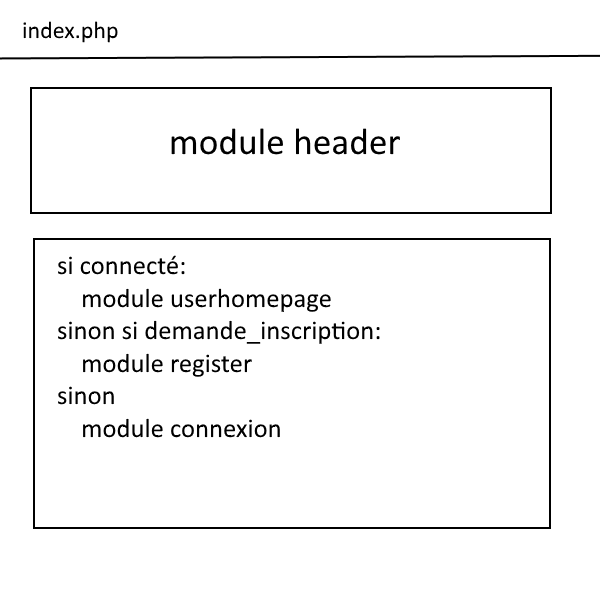
\includegraphics[width=8cm]{index_struct.png}
\end{center}

Chaque module recoit le code javascript et css appelé dans le module head, il est commun. Ils peuvent
aussi avoir leurs propre code qui sera stocké dans \mdbox{modules/js/} et \mdbox{modules/css/}.
Par soucis d'organisation, les scripts propres au module doivent porter le nom de ce dernier. \\
Exemple: \\
Le module \mdbox{modules/foo.php} fait appel à \mdbox{modules/css/foo.css} et \mdbox{modules/js/foo.js}
\\ \\
Le HTML c'est bien, mais la pluspart des balises n'avaient pas vraiment d'utilité, étant donné que l'on
modifiait leurs comportement avec CSS et Javascript quasiment sans arrêt, nous le rappelons, il s'agit là d'une application web. Ainsi, nous n'avons pratiquement utilisé que des \mdbox{DIV},
connaissant leurs propriétés par défaut, il est plus facile de les manipuler par la suite. \\
\\

Le système de connexion est classique et est le seul à rafraichir la page via des formulaires,
toute l'interface du module \mdbox{userhomepage.php} est basé sur des XMLHttpRequests. \\
C'est donc javascript qui se charge de faire des demandes au serveur, 
toutes les demandes javascript sont récéptionnées par des scripts php situés dans \mdbox{requests/}.
\\
Ces scripts réalisent des tâches telles que supprimer un tableau de la base, ajouter un post-it, etc...
\\ \\

Tous les fichiers php peuvent se servir dans \mdbox{scripts/} où des scripts php implémentent des fonctions
récurrentes.

\subsection{Plus en détail}

\subsubsection{Le système de connexion}

\subsubsection{Sauvegarde dynamique}

\subsubsection{Sécurité}

\end{document}
